\begin{figure}[h!]
	\centering
	
	
	\tikzset{every picture/.style={line width=0.75pt}} %set default line width to 0.75pt        
	
	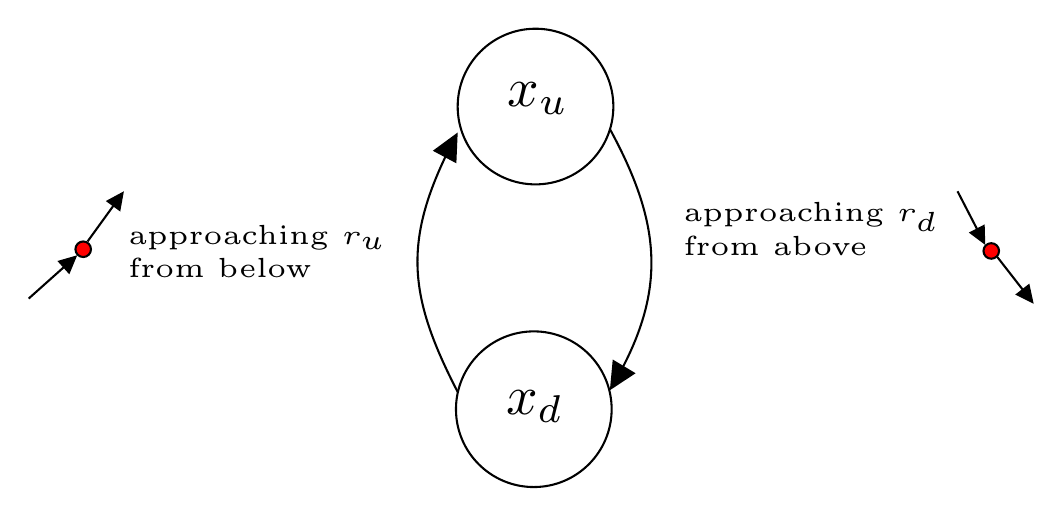
\begin{tikzpicture}[x=0.75pt,y=0.75pt,yscale=-2.5,xscale=2.5]
		%uncomment if require: \path (0,300); %set diagram left start at 0, and has height of 300
		
		%Shape: Circle [id:dp19444798196340818] 
		\draw   (180,45) .. controls (180,36.72) and (186.72,30) .. (195,30) .. controls (203.28,30) and (210,36.72) .. (210,45) .. controls (210,53.28) and (203.28,60) .. (195,60) .. controls (186.72,60) and (180,53.28) .. (180,45) -- cycle ;
		%Shape: Circle [id:dp816887625058681] 
		\draw   (179.67,103.33) .. controls (179.67,95.05) and (186.38,88.33) .. (194.67,88.33) .. controls (202.95,88.33) and (209.67,95.05) .. (209.67,103.33) .. controls (209.67,111.62) and (202.95,118.33) .. (194.67,118.33) .. controls (186.38,118.33) and (179.67,111.62) .. (179.67,103.33) -- cycle ;
		%Curve Lines [id:da5723668381117777] 
		\draw    (180,100) .. controls (170.45,81.54) and (169.41,70.98) .. (178.63,52.64) ;
		\draw [shift={(180,50)}, rotate = 118.07] [fill={rgb, 255:red, 0; green, 0; blue, 0 }  ][line width=0.08]  [draw opacity=0] (5.36,-2.57) -- (0,0) -- (5.36,2.57) -- cycle    ;
		%Curve Lines [id:da3010184020382227] 
		\draw    (210.9,96.96) .. controls (220.24,80.02) and (219.15,67.38) .. (209.33,49.33) ;
		\draw [shift={(209.33,99.67)}, rotate = 300.96] [fill={rgb, 255:red, 0; green, 0; blue, 0 }  ][line width=0.08]  [draw opacity=0] (5.36,-2.57) -- (0,0) -- (5.36,2.57) -- cycle    ;
		%Straight Lines [id:da3364125847880146] 
		\draw    (276.33,61.33) -- (280.29,69) ;
		\draw [shift={(281.67,71.67)}, rotate = 242.7] [fill={rgb, 255:red, 0; green, 0; blue, 0 }  ][line width=0.08]  [draw opacity=0] (3.57,-1.72) -- (0,0) -- (3.57,1.72) -- cycle    ;
		%Shape: Circle [id:dp801346546523267] 
		\draw  [fill={rgb, 255:red, 255; green, 0; blue, 0 }  ,fill opacity=1 ] (281.33,72.83) .. controls (281.33,72) and (282,71.33) .. (282.83,71.33) .. controls (283.66,71.33) and (284.33,72) .. (284.33,72.83) .. controls (284.33,73.66) and (283.66,74.33) .. (282.83,74.33) .. controls (282,74.33) and (281.33,73.66) .. (281.33,72.83) -- cycle ;
		%Straight Lines [id:da3400154107262219] 
		\draw    (284,74) -- (289.16,80.63) ;
		\draw [shift={(291,83)}, rotate = 232.13] [fill={rgb, 255:red, 0; green, 0; blue, 0 }  ][line width=0.08]  [draw opacity=0] (3.57,-1.72) -- (0,0) -- (3.57,1.72) -- cycle    ;
		%Straight Lines [id:da9364634936350018] 
		\draw    (97.33,82) -- (104.43,75.66) ;
		\draw [shift={(106.67,73.67)}, rotate = 138.24] [fill={rgb, 255:red, 0; green, 0; blue, 0 }  ][line width=0.08]  [draw opacity=0] (3.57,-1.72) -- (0,0) -- (3.57,1.72) -- cycle    ;
		%Shape: Circle [id:dp798299245137134] 
		\draw  [fill={rgb, 255:red, 255; green, 0; blue, 0 }  ,fill opacity=1 ] (106.33,72.5) .. controls (106.33,71.67) and (107,71) .. (107.83,71) .. controls (108.66,71) and (109.33,71.67) .. (109.33,72.5) .. controls (109.33,73.33) and (108.66,74) .. (107.83,74) .. controls (107,74) and (106.33,73.33) .. (106.33,72.5) -- cycle ;
		%Straight Lines [id:da06884505715880485] 
		\draw    (108.67,71) -- (113.91,63.76) ;
		\draw [shift={(115.67,61.33)}, rotate = 125.91] [fill={rgb, 255:red, 0; green, 0; blue, 0 }  ][line width=0.08]  [draw opacity=0] (3.57,-1.72) -- (0,0) -- (3.57,1.72) -- cycle    ;
		
		% Text Node
		\draw (186.3,37) node [anchor=north west][inner sep=2.75pt]  [xscale=2,yscale=2] [align=center] {$\displaystyle x_{u}$};
		% Text Node
		\draw (186,96.33) node [anchor=north west][inner sep=2.75pt]  [xscale=2,yscale=2] [align=left] {$\displaystyle x_{d}$};
		% Text Node
		\draw (115.33,66.67) node [anchor=north west][inner sep=0.75pt]  [font=\tiny,xscale=2,yscale=2] [align=left] {approaching $\displaystyle r_{u}$\\from below};
		% Text Node
		\draw (222.33,62.33) node [anchor=north west][inner sep=0.75pt]  [font=\tiny,xscale=2,yscale=2] [align=left] {approaching $\displaystyle r_{d}$\\from above};
		
		
	\end{tikzpicture}
\end{figure}